In this section, we define our neural speaker recognition system and define the targeted and untargeted adversarial attacks we investigate.

\subsection{Neural speaker recognition system}
\label{sub:speaker_recognition}
The speaker recognition system used in our experiments is based on the state-of-the-art framework by \cite{lukic2016speaker} and is described in Figure \ref{fig:CNN}. The first module at the bottom is a pre-processing step that extracts the Mel-Spectrogram from the waveform as described in section \ref{sub:processdata}. The second module is a convolutional neural network (CNN) that performs multi-speaker classification using the Mel-Spectrogram. The CNN is a modified version of Alexnet~\cite{krizhevsky2012imagenet}. We warn the readers that unlike ~\ref{fig:CNN}, our classifier operates on 64 by 64 Mel -Spectrogram and has slightly different number of nodes on each layer.

\begin{figure}[h]
    \centering
    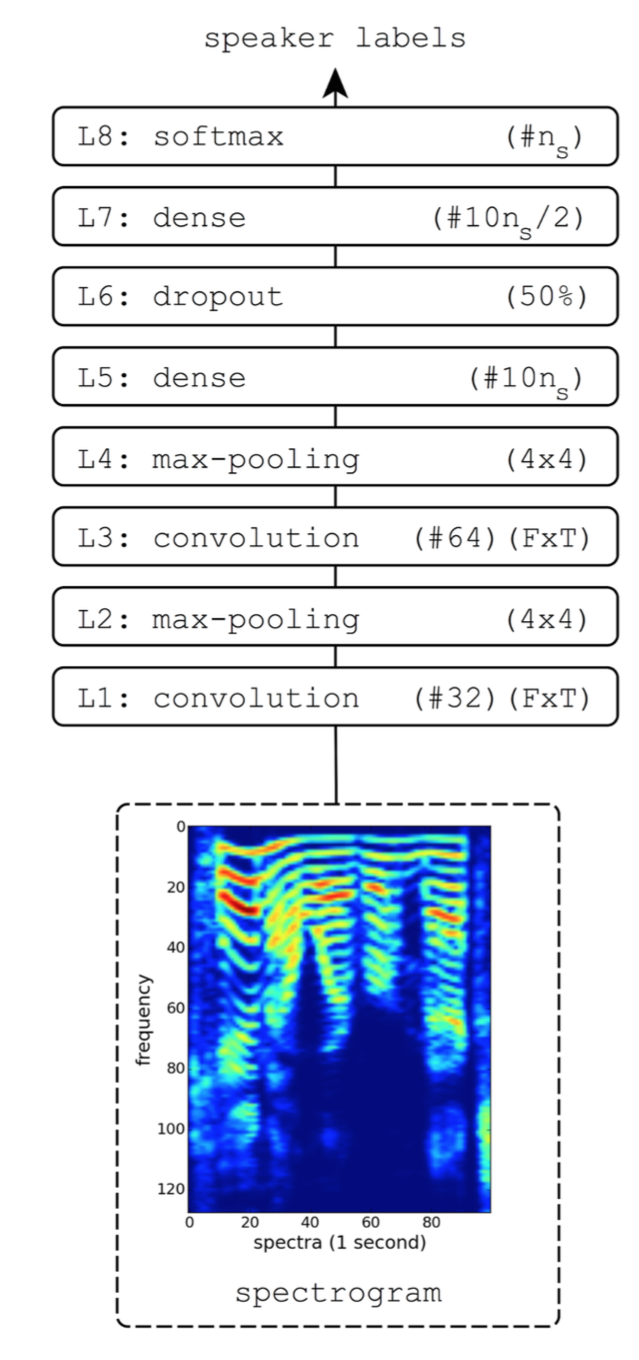
\includegraphics[width=0.25\textwidth]{./fig/cnn.png}
    \caption{Architecture for CNN speaker verifier}
    \label{fig:CNN}
\end{figure}

We train the CNN on our training set using 64 by 64 Mel-Spectrograms~\footnote{64 mel bands and 64 frames, 100 ms each} consisting of balanced samples from 102 speakers from the NIST 2004, Blizzard, and VCTK(P280) datasets. Our model achieves 85\% test set accuracy.

\subsection{Adversarial attacks}
We define adversarial attacks on speaker recognition systems as \textit{targeted} or \textit{untargeted}. In
targeted attacks, an adversary is interested in designing an input
that makes the classification system predict a target class chosen by the
adversary. In untargeted attacks, the adversary is interested in a confident
prediction, regardless of the class being predicted. Untargeted attacks are essentially designed to fool the classifier into thinking a fake speech sample is real. Notice that a successful targeted attack is by definition a successful untargeted attack as well.